\documentclass{acmtog}

%%%%%%%%%%%%%%%%%%%%%%
% PACKAGES
%

\usepackage[utf8]{inputenc}

\usepackage{graphicx}

\usepackage{todonotes}
\newcommand{\todoin}[1]{\todo[inline]{#1}}

\usepackage{indentfirst}
\usepackage{hyperref}
\usepackage{cleveref}
\usepackage{url}
\usepackage{breakurl}

\usepackage{natbib}


%%%%%%%%%%%%%%%%%%%%%%

\acmVolume{}
\acmNumber{}
\acmYear{2012}
\acmMonth{July}
\acmArticleNum{}  
\acmdoi{}

\begin{document}

\markboth{Pedro Costa}{A Review on GPU Accelerated Pathfinding}

\title{A Review on GPU Accelerated Pathfinding} % title

\author{PEDRO~COSTA%
\affil{Universidade~do~Minho}}

% \category{I.3.7}{Computer Graphics}{Three-Dimensional Graphics and Realism}[Animation]
% \category{I.3.5}{Computer Graphics}{Computational Geometry and Object Modeling}[Physically based modeling]

\category{G.2.2}{Discrete Mathematics}{Graph Theory}[Path and circuit problems]
\category{I.2.1}{Artificial Inteligence}{Applications and Expert Systems}[Games]
\category{I.2.8}{Artificial Inteligence}{Problem Solving, Control Methods, and Search}[Graph and tree search strategies,Heuristic methods]
\category{I.2.9}{Artificial Inteligence}{Robotics}

\category{I.3.1}{Computer Graphics}{Hardware Architecture}[Graphics processors]

% \terms{Experimentation, Human Factors}
\terms{Pathfinding}

% \keywords{Face animation, image-based modelling, iris animation, photorealism, physiologically-based modelling}
\keywords{CUDA, A star, Dijkstra, artificial inteligence}

% \acmformat{Avi Bleiweiss. 2008. GPU accelerated pathfinding. In Proceedings of the 23rd ACM SIGGRAPH/EUROGRAPHICS symposium on Graphics hardware (GH '08). Eurographics Association, Aire-la-Ville, Switzerland, Switzerland, 65-74.}

\maketitle

\begin{bottomstuff} 
P. Costa is a student in the Master's Degree of Informatics Engineering at the Department of Informatics. This document was written in the scope of the Virtual and Augmented Reality module for the Curricular Specialization Unit of Computer Graphics.

Author address: \texttt{pg19830@alunos.uminho.pt}
\end{bottomstuff}


\begin{abstract}
\todoin{Abstract missing}
\end{abstract}

\section{Introduction}
\section{Pathfinding}

Solving the pathfinding problem involves two distinct steps.
First, a graph must be built, representing the possible paths an agent can take.
This allows to immediatly take in consideration static obstacles in a global fashion, at least for all the agents that follow a specific graph.
Second, a search algorithm must be used to search the best route along the created graph.

In \cite{johansson09} many approaches to the graph used in the pathfinding problem are described:
\begin{description}
	\item [Grid-based] The space is regularly divided in tiles. Each tile is evaluated to see if it has an obstacle, before moving to that tile. Easy to implement but creates unrealistic paths.
	\item [Roadmap] A graph, representing the possible movements an agent may perform, is created. It does not find the optimal routes and may not create a realistic path. Also, usually the roadmaps are manually defined.
	\item [Visibility Graphs] The corners of the objects are the nodes of the graph. Two nodes are linked if no obstacle exists between them. Causes wall-hugging, which creates paths far from natural.
	\item [Corridor Map] A more modern approach to roadmaps. A graph is built, representing the possible corridors. The path is estimated along the graph. Each point of the path is linked to the nearest obstacles to provide some safe colision distance. Triangulation provides the best route along the estimated path, creating realistic movements. 
\end{description}

As for the search algorithm, the most common approach is the A$\star$ algorithm.
Similar to the more commonly known \textit{Dijkstra} algorithm, it searches for the best (shortest) path from an initial point to a goal.
The two algorithms differ in the existence of an heuristic.
The A$\star$ algorithm chooses the next step by considering the cost of reaching the next point and the estimate of the total cost from that point to the goal (given by the heuristic function).
This is usually a distance function (\textit{Manhattan}, \textit{Euclidean}).

The \textit{Dijkstra} algorithm is very irregular and divergent, which does not favor its implementation in the GPU.
The A$\star$ suffers from similar problems, but since it requires more arithmetic operations per node, it is expected to achieve better performance.
\section{Implementation}

\cite{bleiweiss08} describes the implementation of a library for motion planning using CUDA in the GPU.

The graph is represented as a roadmap implemented using an adjacency list. Dynamic roadmaps, which change over time were not focused. Being static, the roadmap was stored in the GPU using textures memory since it is read-only and cached.

The search algorithm A$\star$ was implemented as an independent kernel. The inputs of this kernel were defined in a \textit{Structs-Of-Arrays} approach, which favors coalesced accesses:
\begin{itemize}
	\item One path per agent (defined as start and goal points);
	\item Costs from the start position (initialized at zero);
	\item Combined costs (estimated, from start to goal, initialized at zero);
	\item A pair of arrays holding the pending and shortest edge collections.
\end{itemize}

One of the improvements added to the A$\star$ algorithm was the implementation of a node priority queue, which allows the best nodes to be placed on top, despite the order of insertion.
The priority queue was implemented as an inline heap, with two optimized GPU kernels for insertion and extraction (and removal).

The GPU hardware used in \cite{bleiweiss08} had a very small amount of memory (512 MB). The author worked around this limitation by splitting the computation into a sequence of multi launch tasks. Between each launch, the partial result is written in the larger host memory.

Each thread in the GPU simulated a single agent.
\section{Results}

The implemented library was tested using several undirected roadmaps (with $N$ nodes), each using $N^2$ agents.

The benchmarks were performed using two distinct CPU versions (a C++ scalar optimized with O2 version, and a manually tuned SIMD version) and the GPU version already described. CPU tests were performed using a single core processor and a dual processor single core machine. Also, the library was tested using both the A$\star$ algorithm and the \textit{Dijkstra} algorithm (no heuristic).

The GPU version achieved a speedup of 27 against the CPU scalar C++ optimized version (\textit{Dijkstra} algorithm).Using the A$\star$ algorithm with an Euclidean distance heuristic, it achieved a speedup of around 55 compared to the CPU, due to the presence of more arithmetic computations per node.
This improvement was already expected due to the more arithmetic intense behaviour of the A$\star$.

The dual processor SSE implementation obtained a speedup of 2.3 against the C++ scalar O2 version. Compared to the SIMD version, the CUDA implementation using the A$\star$ algorithm reached a speedup of 24.

\begin{figure}[!htp]
	\centering
	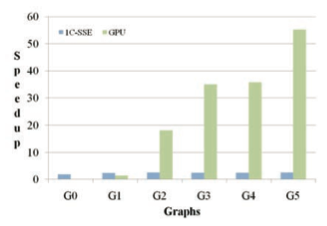
\includegraphics[width=\columnwidth]{images/speedups.png}
	\caption{Best results achieved (image from the original paper). The original caption states that these results reveal the speedup obtained with the CUDA implementation compared to the two sequential versions. Yet, the legend in the chart and the results text in the paper leads to the conclusion that these results are for the CUDA and SSE implementations against the C++ scalar O2 version.}
\end{figure}
\section{Conclusion}

\cite{bleiweiss08} has successfully proven that an irregular and divergent algorithm such as A$\star$, with a small set of tweaks, could effectively obtain speedups running in a GPU architecture, where this characteristics are harmfull.

The author has further developed the pathfinding library applied to the GPU in \cite{bleiweiss09}. \cite{inam10} also optimized the original implementation of th A$\star$ algorithm in the GPU architecture. This library is publicly available in the NVidia website for developpers.

Although the benefits of using the A$\star$ algorithm in a GPU architecture were demonstrated in the reviewed document, \cite{johansson09} questions \citeauthor{bleiweiss08}'s decision to perform tests with a large number of agents and a few nodes.
While the scope of the author's work is in improving artificial inteligence features using CUDA, in a game environment it is most common to exist a reasonably low number of agents, and thousands of possible points in their routes. This question remains unanswered in \cite{bleiweiss09}.

Although the basis of this work produced proven results, the comparisons performed in the benchmarks are outdated and were slightly bias. Two very distinct CPUs with very small parallel capabilities were used. Due to the already mentioned characteristics of the algorithm, a modern CPU with a high parallel capability should be able to nearly match the results obtained with the GPU hardware described in \cite{bleiweiss08}. On the other hand, GPU hardware has greatly evolved since the article was published. Among other characteristics, GPUs have much more memory, and are able to compute using double precision floating-point numbers. Finally, distributed memory approaches were already available at the time of the paper, and could greatly boost the CPU versions, but no tests were performed using it.

A more up-to-date approach to this problem can be found in \cite{inam10}, although the authors only explore the implementation of the A$\star$ algorithm in a GPU, instead of the whole pathfinding system.

\bibliographystyle{acmtog}
\bibliography{bib/article,bib/inproceedings,bib/misc}

\end{document}
